%Para hacer informe con portada utilizamos report

\documentclass[12pt]{report}

\usepackage[a4paper]{geometry}
\usepackage[myheadings]{fullpage}
\usepackage{fancyhdr}
\usepackage{lastpage}
\usepackage{graphicx, wrapfig, subcaption, setspace, booktabs}
\usepackage[T1]{fontenc}
\usepackage[font=small, labelfont=bf]{caption}
\usepackage{fourier}
\usepackage[protrusion=true, expansion=true]{microtype}

%Paquete para hipervinculos
\usepackage[colorlinks=true]{hyperref}
\hypersetup{
    colorlinks=true,
    linkcolor=black,
    filecolor=magenta,      
    urlcolor=blue,
}

%Para qué los subtítulos aparezcan en español
\usepackage[spanish]{babel}
\usepackage[utf8]{inputenc}
\usepackage{sectsty}
\usepackage{url, lipsum}
\usepackage{tabularx}
\usepackage{float}

%--------------------------------------------------
%Para agregar citas en apa
%Para citar se usa el comando \cite{}
%Las referencias se modifican en el archivo sample.bib
\usepackage{apacite}
%----------------------------------------------

\newcommand{\HRule}[1]{\rule{\linewidth}{#1}}
\onehalfspacing
\setcounter{tocdepth}{5}
\setcounter{secnumdepth}{5}

%-------------------------------------------------------


\begin{document}


%-------------------------------------------------------------------------------
% Portada
%-------------------------------------------------------------------------------
\begin{titlepage}
    \begin{center}
        \vspace*{1cm}
            
        \Huge
        \textbf{Nociones de la memoria del computador}
            
        \vspace{0.5cm}
        \LARGE
        
            
        \vspace{1.5cm}
            
        \textbf{Geraldine Ramirez Londoño }
            
        \vfill
            
        \vspace{0.8cm}
            
        \Large
        Despartamento de Ingeniería Electrónica y Telecomunicaciones\\
        Universidad de Antioquia\\
        Medellín\\
        Septiembre de 2020
            
    \end{center}
\end{titlepage}
\newpage

\tableofcontents
%-------------------------------------------------------
\newpage
\section{Introducción}


En este documento hablaremos un poco acerca de la memoria del computador , los tipos de memoria , y la menera en que estos  permiten el correcto funcionamiento del computador.

\section{La memoria del computador }
primero hablemos un poco acerca de la memoria del computador.
Podríamos decir que la memoria de el computador es uno de los elementos más importantes para que todo funcione correctamente, es más, sin ella el PC ni siquiera podría arrancar.Tal es la importancia que este componente electrónico tiene en la estructura de nuestro computador.
Pero antes de adentrarnos en cuestiones de rendimiento y capacidades de la memoria, debemos tener en cuenta que la palabra “Memoria” es un término genérico usado para designar las partes del computador o de los dispositivos periféricos donde todos los datos y programas son almacenados.

\section{Tipos de memoria}
Una computadora trabaja al menos con cuatro tipos de memoria diferentes, y cada una de ellas se encarga de realizar una función distinta. Estas son la memoria RAM, memoria ROM, la memoria SRAM o Caché, la memoria Swap o Virtual, entre otras.

 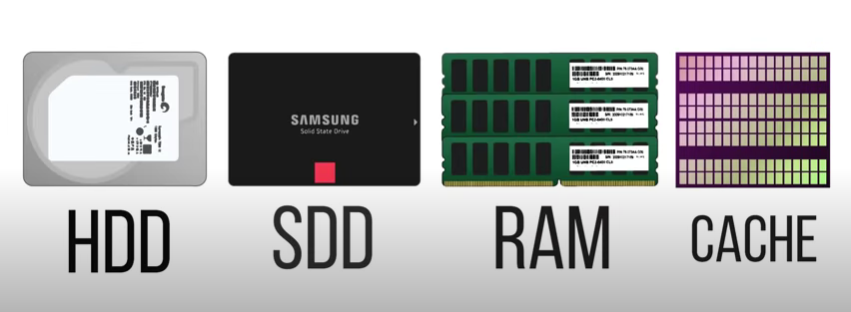
\includegraphics[width=1.00\textwidth]{MEMORIAS.PNG}
 
 \begin{itemize}
        \item { Memoria HHD (diso duro o estado solido )}
        siendo uno de los companentes mas importante de cualquier sistema informatico el disco duro es un dispositivos de almacenamiento de datos en el cual podemos almacenar cualquier tipo de información digital. Ya sean fotografías, vídeos, archivos de texto o programas informáticos
        
        en cuanto a su funcionamiento este tiene varios discos adentro y cada vez que se solicita un archivo debe buscarlo dentro de estos discos, tiene una tabla donde esta apuntado  el sitio de cada uno de estos archivos, el cual llama “Sistema de ficheros “  y luego procede a buscar los datos en la posición indicada
        
         \item { Memoria SSD (unidad de estado sólido)} Cumple con la función de almacenar datos de tu ordenador. Básicamente, un SSD hace lo mismo que un HDD, La gran diferencia es que mientras los discos duros utilizan componentes mecánicos que se mueven, las SSD almacenan los archivos en microchips con memorias flash interconectadas entre sí.
        
         \item { Memoria RAM (memoria principal) }la memoria RAM, es el área de trabajo del ordenador y en ella se encuentran tanto las instrucciones  como los datos que está utilizando el procesador o el CPU del ordenador para trabajar
        
         \item { Memoria SRAM (memoria cache)} la memoria cache es el área de almacenamiento dedicada a los datos usados o solicitados con más frecuencia para su recuperación a gran velocidad. Podemos decir que esta es un paso intermedio entre la RAM y la memoria del procesador
        
         \item { Memoria VRAM (memoria de la tarjeta gráfica)}
        Es un tipo de memoria diseñada para llevar a cabo tareas específicas como aplicaciones diseño o videojuegos permite descargar muchos datos al mismo tiempo, pero al momento de buscar los datos demora en encontrarlos. 
  
        \item { Memoria ROM (Memoria de Sólo Lectura)}  esta se utiliza para almacenar los programas que ponen en marcha nuestro equipo, sirve para las diversas rutinas de control en los dispositivos de entrada y salida 
        Se caracteriza por ser una memoria volátil, a diferencia de la RAM es mucho más lenta para acceder a la información, ya que es secuencial (necesita recorrer todos los datos hasta hallar la información) 
        
         \item { Memoria VIRTUAL} no tiene un lugar específico en la máquina. 
        Se utiliza  cuando hay mucha información en la memoria RAM, para compensar la falta de memoria y poder acelerar los procesos, toma archivos de la RAM y los lleva al disco rígido, creando una carpeta de datos 


 \cite{tipos}
 \cite{memoria}


\end{itemize}





\section{gestion de la memoria en un computador.} 

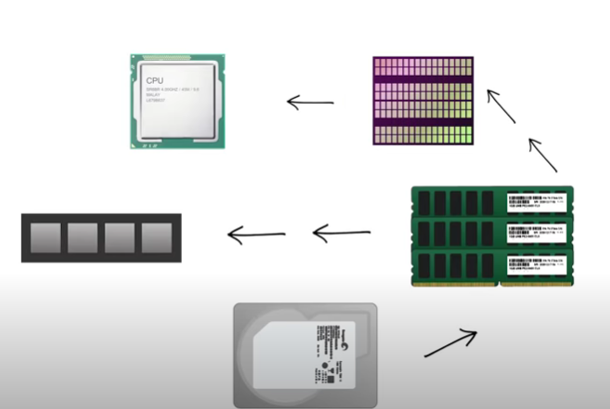
\includegraphics[width=1.00\textwidth]{imagen 2.PNG}
\vspace{0.1cm}

Cada memoria del computador cumple con una función de acuerdo a sus capacidades, considerando que la memoria RAM es mucho más rápida que el disco  y para que el procesador no se quede esperando que los datos carguen desde el disco se utiliza la RAM, pero si utilizamos solo esta memoria el computador puede presentar intermitencias  en algunas ocasiones. Para esto se introdujo otro nivel de memoria llamado SRAM o memoria cache, este es un paso intermedio entre la RAM y el procesador; su principal función consiste en tener a la mano los procesos que se realizan de manera recurrente; por este motivo cuando  el procesador necesita buscar archivos se dirige en primer lugar a la memoria cache  y luego como segunda opción esta la memoria RAM, por último y en caso tal de no encontrar la información en las memorias anteriores este se dirige al disco duro y así se repite el proceso de intercambio de información entre ellos, hasta el momento en que el computador se apaga.


\section{¿Qué hace que una memoria sea más rápida que otra? ¿Por qué esto es importante?}

La velocidad de una memoria depende tanto de las especificaciones físicas como digitales, La memoria RAM y el disco duro se utilizan para almacenar información pero su función dentro de un PC es muy diferente. En pocas palabras, la memoria RAM es una memoria de trabajo pero su capacidad de almacenamiento es inferior en comparación con el disco duro, el cual es una memoria de almacenamiento con grandes limitaciones en cuanto a su capacidad para encontrar información a tiempo; pero tanto el disco duro como la memoria RAM cumple una función muy importante en el computador una no podría funcionar sin la ayuda de la otra, cada una cumple con función especifica tanto la memoria ROM,VRAM y cache son importante para asegurar el rendimiento de la velocidad en el computador; si pudiéramos tener una memoria que tenga  tanto velocidad como almacenamiento no sería necesario el uso de tantas memorias  para permitir un buen funcionamiento en el computador, posiblemente en el futuro esto sea posible pero por ahora el uso de estas es completamente necesario



\section{Conclusión} \label{conclulsion}
Algunas memorias son lentas pero fiables, otras son rápidas pero olvidadizas, otras mucho más rápidas pero voluminosas, mientras que otras pueden proveer más datos a la vez pero demoran más por cada lectura, en fin cada memoria tiene sus pros y sus contras, por ese motivo nuestro computador  utiliza tantas.



\newpage

\bibliographystyle{apacite}
\bibliography{sample.bib}


\end{document}


